\documentclass[twoside]{book}

% Packages required by doxygen
\usepackage{fixltx2e}
\usepackage{calc}
\usepackage{doxygen}
\usepackage[export]{adjustbox} % also loads graphicx
\usepackage{graphicx}
\usepackage[utf8]{inputenc}
\usepackage{makeidx}
\usepackage{multicol}
\usepackage{multirow}
\PassOptionsToPackage{warn}{textcomp}
\usepackage{textcomp}
\usepackage[nointegrals]{wasysym}
\usepackage[table]{xcolor}

% Font selection
\usepackage[T1]{fontenc}
\usepackage[scaled=.90]{helvet}
\usepackage{courier}
\usepackage{amssymb}
\usepackage{sectsty}
\renewcommand{\familydefault}{\sfdefault}
\allsectionsfont{%
  \fontseries{bc}\selectfont%
  \color{darkgray}%
}
\renewcommand{\DoxyLabelFont}{%
  \fontseries{bc}\selectfont%
  \color{darkgray}%
}
\newcommand{\+}{\discretionary{\mbox{\scriptsize$\hookleftarrow$}}{}{}}

% Page & text layout
\usepackage{geometry}
\geometry{%
  a4paper,%
  top=2.5cm,%
  bottom=2.5cm,%
  left=2.5cm,%
  right=2.5cm%
}
\tolerance=750
\hfuzz=15pt
\hbadness=750
\setlength{\emergencystretch}{15pt}
\setlength{\parindent}{0cm}
\setlength{\parskip}{3ex plus 2ex minus 2ex}
\makeatletter
\renewcommand{\paragraph}{%
  \@startsection{paragraph}{4}{0ex}{-1.0ex}{1.0ex}{%
    \normalfont\normalsize\bfseries\SS@parafont%
  }%
}
\renewcommand{\subparagraph}{%
  \@startsection{subparagraph}{5}{0ex}{-1.0ex}{1.0ex}{%
    \normalfont\normalsize\bfseries\SS@subparafont%
  }%
}
\makeatother

% Headers & footers
\usepackage{fancyhdr}
\pagestyle{fancyplain}
\fancyhead[LE]{\fancyplain{}{\bfseries\thepage}}
\fancyhead[CE]{\fancyplain{}{}}
\fancyhead[RE]{\fancyplain{}{\bfseries\leftmark}}
\fancyhead[LO]{\fancyplain{}{\bfseries\rightmark}}
\fancyhead[CO]{\fancyplain{}{}}
\fancyhead[RO]{\fancyplain{}{\bfseries\thepage}}
\fancyfoot[LE]{\fancyplain{}{}}
\fancyfoot[CE]{\fancyplain{}{}}
\fancyfoot[RE]{\fancyplain{}{\bfseries\scriptsize Generated by Doxygen }}
\fancyfoot[LO]{\fancyplain{}{\bfseries\scriptsize Generated by Doxygen }}
\fancyfoot[CO]{\fancyplain{}{}}
\fancyfoot[RO]{\fancyplain{}{}}
\renewcommand{\footrulewidth}{0.4pt}
\renewcommand{\chaptermark}[1]{%
  \markboth{#1}{}%
}
\renewcommand{\sectionmark}[1]{%
  \markright{\thesection\ #1}%
}

% Indices & bibliography
\usepackage{natbib}
\usepackage[titles]{tocloft}
\setcounter{tocdepth}{3}
\setcounter{secnumdepth}{5}
\makeindex

% Hyperlinks (required, but should be loaded last)
\usepackage{ifpdf}
\ifpdf
  \usepackage[pdftex,pagebackref=true]{hyperref}
\else
  \usepackage[ps2pdf,pagebackref=true]{hyperref}
\fi
\hypersetup{%
  colorlinks=true,%
  linkcolor=blue,%
  citecolor=blue,%
  unicode%
}

% Custom commands
\newcommand{\clearemptydoublepage}{%
  \newpage{\pagestyle{empty}\cleardoublepage}%
}

\usepackage{caption}
\captionsetup{labelsep=space,justification=centering,font={bf},singlelinecheck=off,skip=4pt,position=top}

%===== C O N T E N T S =====

\begin{document}

% Titlepage & ToC
\hypersetup{pageanchor=false,
             bookmarksnumbered=true,
             pdfencoding=unicode
            }
\pagenumbering{alph}
\begin{titlepage}
\vspace*{7cm}
\begin{center}%
{\Large My F\+EM Project }\\
\vspace*{1cm}
{\large Generated by Doxygen 1.8.14}\\
\end{center}
\end{titlepage}
\clearemptydoublepage
\pagenumbering{roman}
\tableofcontents
\clearemptydoublepage
\pagenumbering{arabic}
\hypersetup{pageanchor=true}

%--- Begin generated contents ---
\chapter{Main Page}
\label{index}\hypertarget{index}{}\section*{F\+E\+Mproject}

Trabaho Final da Disciplina de Introdução ao Método dos Elementos Finitos

\section*{Autores}


\begin{DoxyItemize}
\item Igor de Melo Nery de Oliveira
\item Lucas Gouveia Omena Lopes
\end{DoxyItemize}

\section*{Projeto Final}


\begin{DoxyItemize}
\item Implementação dos Elementos Finitos Q4 e T6 para resolução de um problema de uma estrutura submetida ao estado plano de tensões.
\end{DoxyItemize}

\section*{Problema Estudado}

Pilar engastado na base, e submetido a uma carga distribuída vertical no topo\+:

\subsection*{html /\+Figuras/problema.png}


\begin{DoxyImageNoCaption}
  \mbox{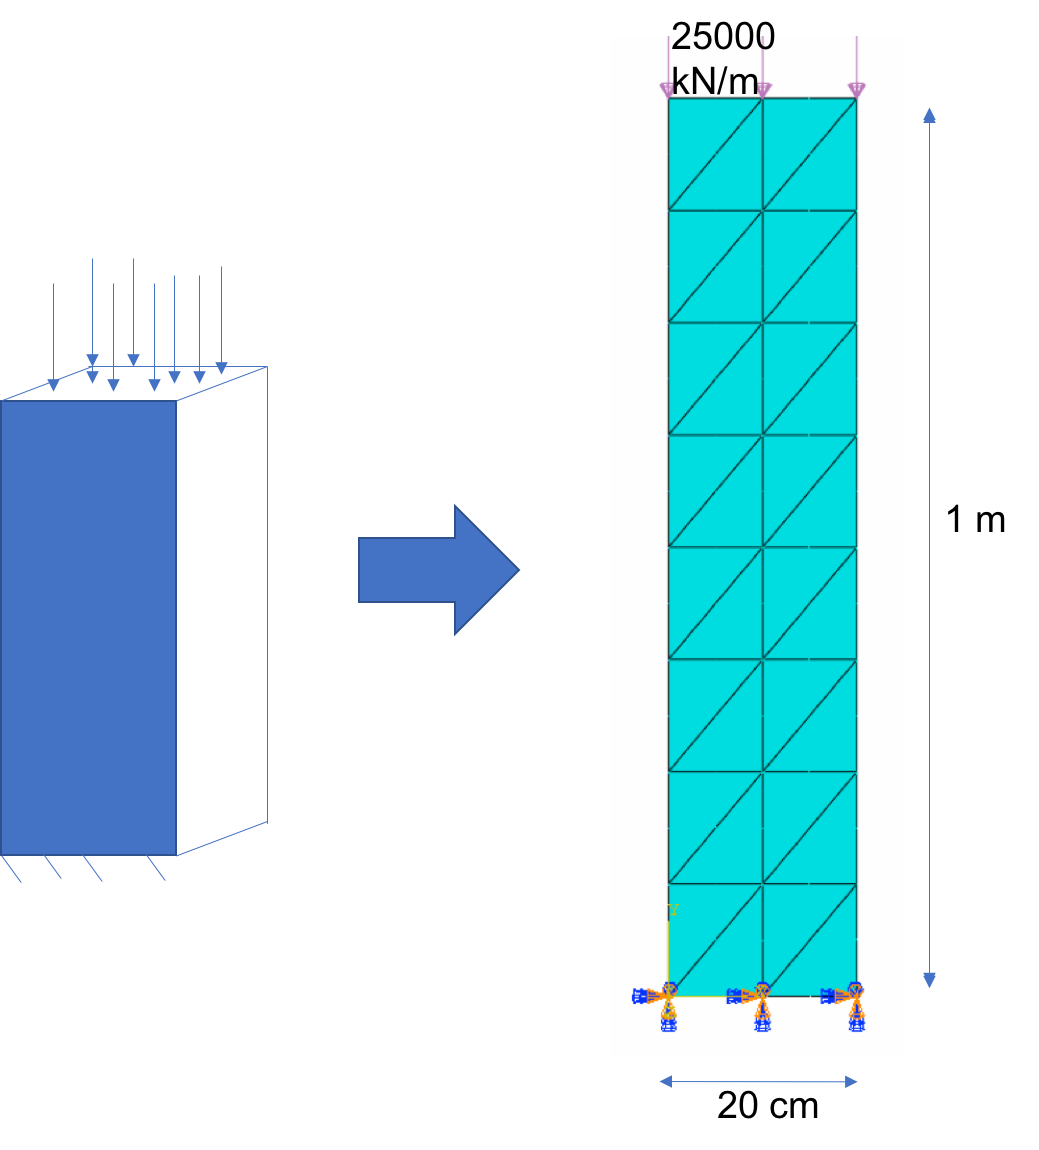
\includegraphics[width=\textwidth,height=\textheight/2,keepaspectratio=true]{problema.png}}
\end{DoxyImageNoCaption}
 

\section*{Elementos em Estudo}

\subparagraph*{Elemento Q4\+:}


\begin{DoxyItemize}
\item Elemento Quadilateral de 4 nós
\end{DoxyItemize}

\subsection*{html /\+Figuras/element\+Q4.png}


\begin{DoxyImageNoCaption}
  \mbox{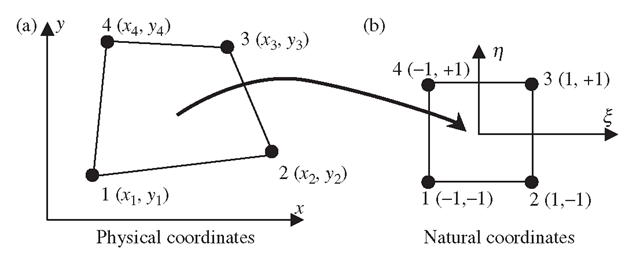
\includegraphics[width=\textwidth,height=\textheight/2,keepaspectratio=true]{elementQ4.png}}
\end{DoxyImageNoCaption}
 

\subparagraph*{Elemento T6\+:}


\begin{DoxyItemize}
\item Elemento Triangular de 6 nós
\end{DoxyItemize}

\subsection*{html /\+Figuras/\+T6.png}


\begin{DoxyImageNoCaption}
  \mbox{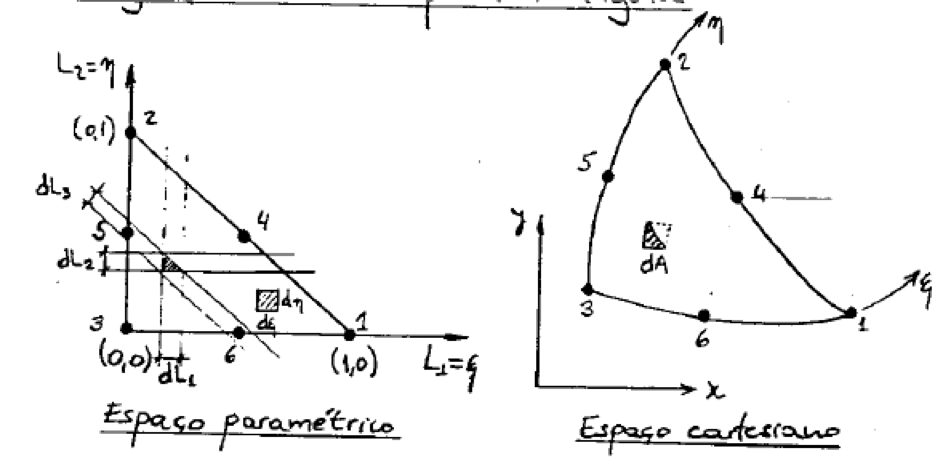
\includegraphics[width=\textwidth,height=\textheight/2,keepaspectratio=true]{T6.png}}
\end{DoxyImageNoCaption}
 

\section*{Objetivos}


\begin{DoxyItemize}
\item Implementação e uso dos elementos Q4 e T6 na resolução do problema proposto;
\item Avaliação dos resultadsos e comparação dos mesmos com os do software Abaqus.
\end{DoxyItemize}

\section*{Resultados}

\subsection*{Implementação Computacional dos Elementos T6 e Q4}


\begin{DoxyItemize}
\item As implementações dos elementos, juntamente com um código de análise de problemas usando o Método dos Elementos Finitos, foram feitas fazendo-\/se uso da linguagem de programação C++;
\item Os códigos e documentações seguem junto a esse P\+DF, podendo ser acessados de maneira iterativa através do arquivo H\+T\+ML, onde toda documentação e comentários se encontram.
\item A implementação apresentada faz uso do arquivo de entrada do software comercial Abaqus, afim de tirar proveito da ferramenta de geração de malhas do mesmo;
\item Os resultados obtidos através dessa implementação são verificados através do Abaqus, e serão apresentados posteriormente.
\end{DoxyItemize}

\subsection*{Abaqus}


\begin{DoxyItemize}
\item Foram testados exemplos, utilizando como material o aço (Modulo de Young 200 G\+Pa e coeficiente de Poisson 0.\+3), e estudados os efeitos do tipo de elemento e refinamento da malha nos resultados obtidos. Esses resultados, visulaizados através das ferramentas do software Abaqus. Os campos avaliados foram os deslocamentos (U),tensões (S), reações de apoio (RF) e deformações na estrutura (E).
\end{DoxyItemize}

\subsubsection*{Deslocamentos}

\subsubsection*{html /\+Figuras/45U.png}


\begin{DoxyImageNoCaption}
  \mbox{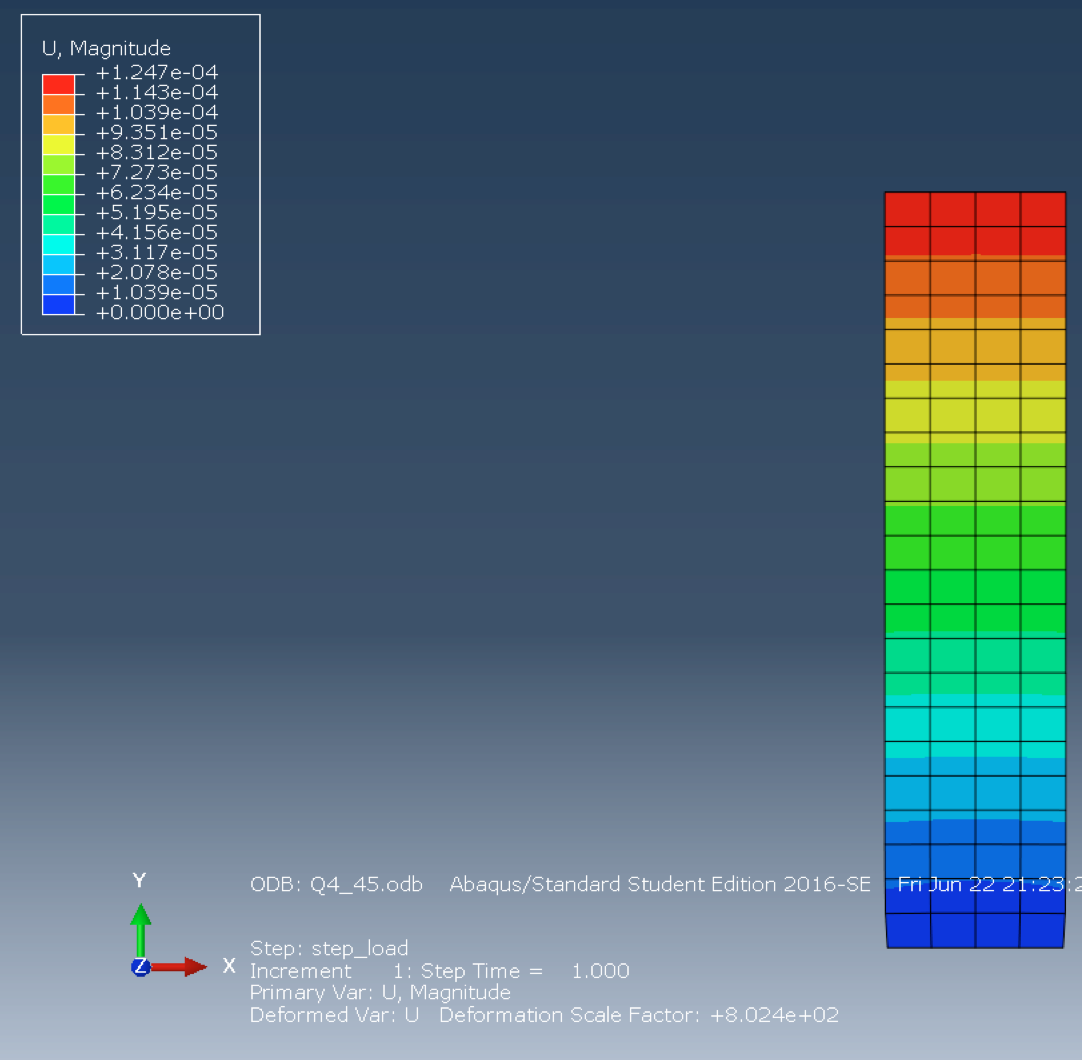
\includegraphics[width=\textwidth,height=\textheight/2,keepaspectratio=true]{45U.png}}
\end{DoxyImageNoCaption}
 

\subsubsection*{Tensões}

\subsubsection*{html /\+Figuras/45S.png}


\begin{DoxyImageNoCaption}
  \mbox{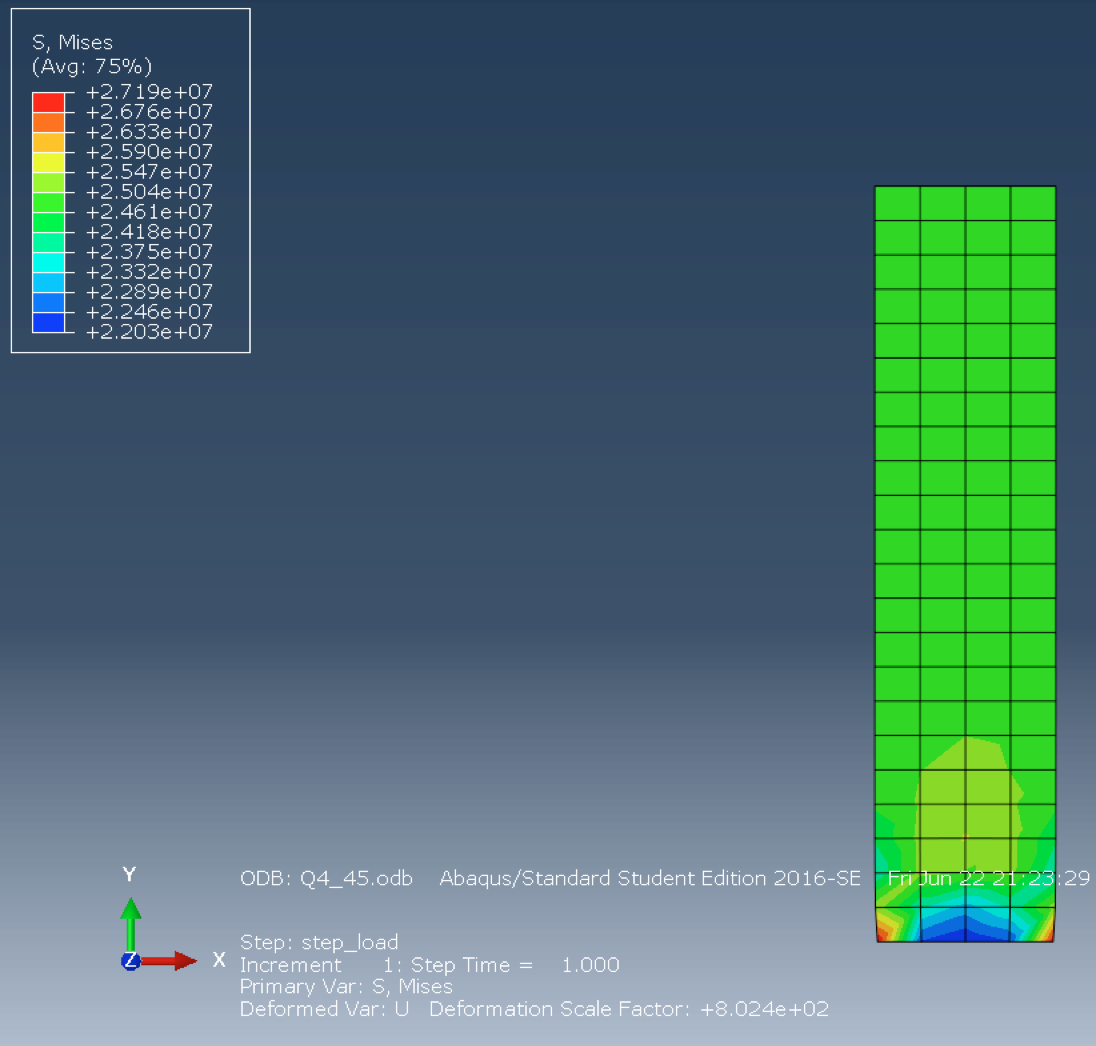
\includegraphics[width=\textwidth,height=\textheight/2,keepaspectratio=true]{45S.png}}
\end{DoxyImageNoCaption}
 

\subsubsection*{Reações}

\subsubsection*{html /\+Figuras/45\+RF.png}


\begin{DoxyImageNoCaption}
  \mbox{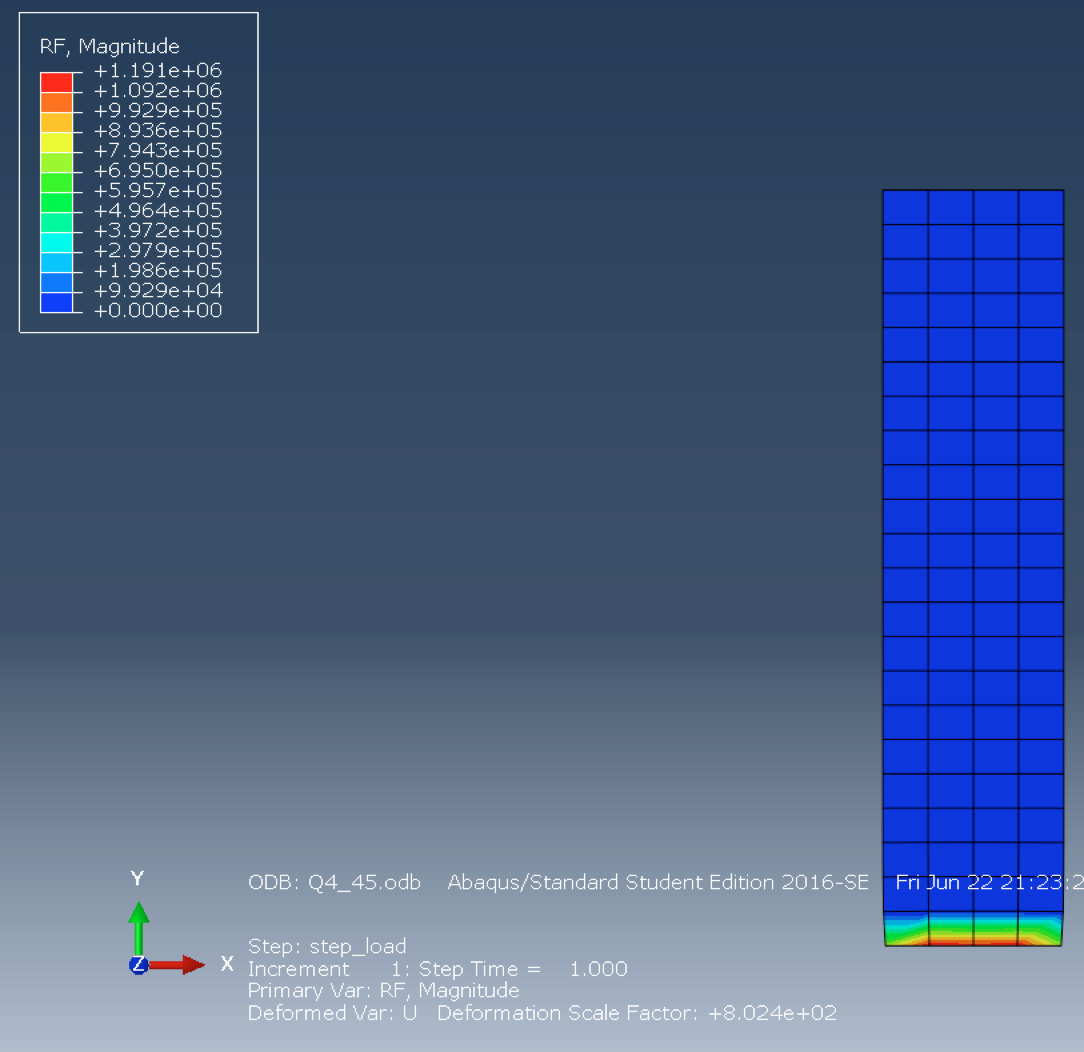
\includegraphics[width=\textwidth,height=\textheight/2,keepaspectratio=true]{45RF.png}}
\end{DoxyImageNoCaption}
 

\subsubsection*{Deformações}

\subsubsection*{html /\+Figuras/45E.png}


\begin{DoxyImageNoCaption}
  \mbox{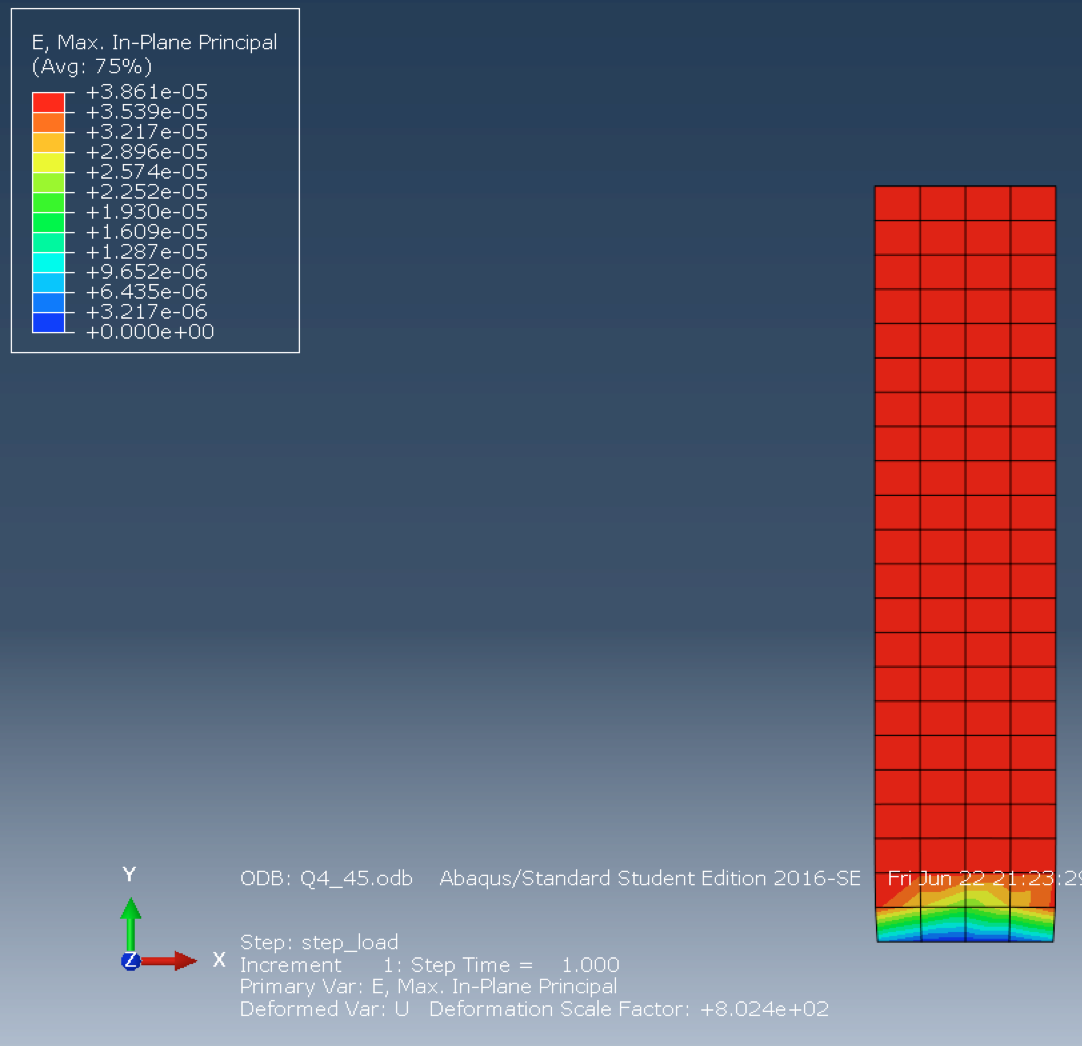
\includegraphics[width=\textwidth,height=\textheight/2,keepaspectratio=true]{45E.png}}
\end{DoxyImageNoCaption}
 

\subsection*{Influência do Número de Elementos}


\begin{DoxyItemize}
\item Para avaliarmos a interferência do refinamento da malha nos resultados obtidos, realizou-\/se um estudo das tensões e deformações medidas nos elementos. Esse estudo pode ser fisto nas figuras a seguir (simulações do Abqus para variadas divisões de elementos), e no gráfico, que mostra a influência do resultado de acordo com o número de elementos.
\end{DoxyItemize}

\subsubsection*{html /\+Figuras/tabela.png}


\begin{DoxyImageNoCaption}
  \mbox{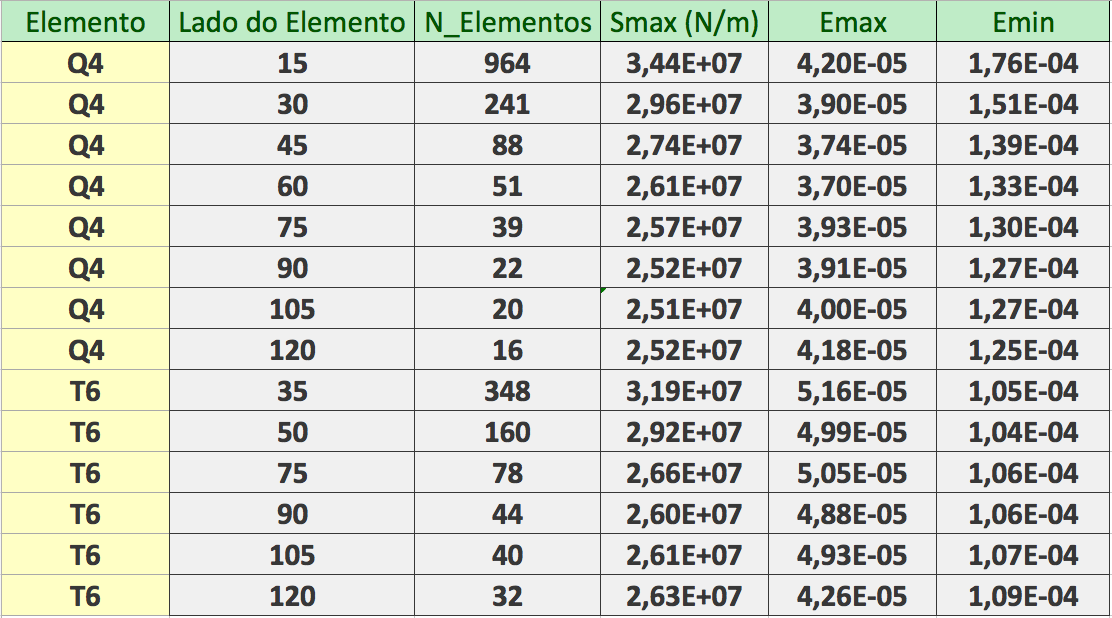
\includegraphics[width=\textwidth,height=\textheight/2,keepaspectratio=true]{tabela.png}}
\end{DoxyImageNoCaption}
 

\subsubsection*{Q4}

\subsubsection*{html /\+Figuras/stress.png}


\begin{DoxyImageNoCaption}
  \mbox{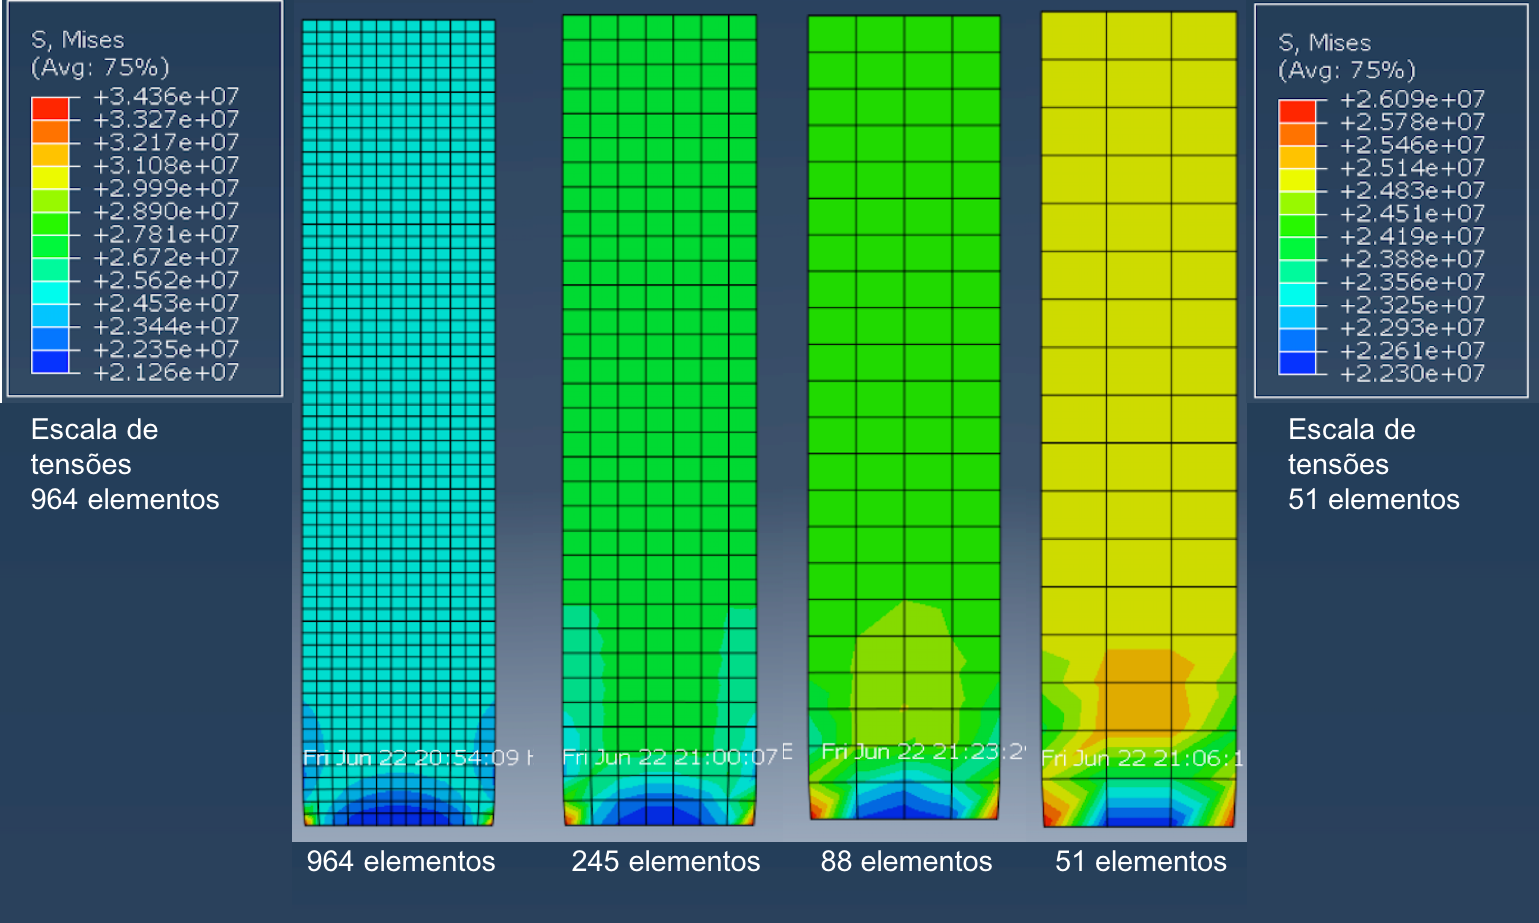
\includegraphics[width=\textwidth,height=\textheight/2,keepaspectratio=true]{stress.png}}
\end{DoxyImageNoCaption}
 

\subsubsection*{html /\+Figuras/strain.png}


\begin{DoxyImageNoCaption}
  \mbox{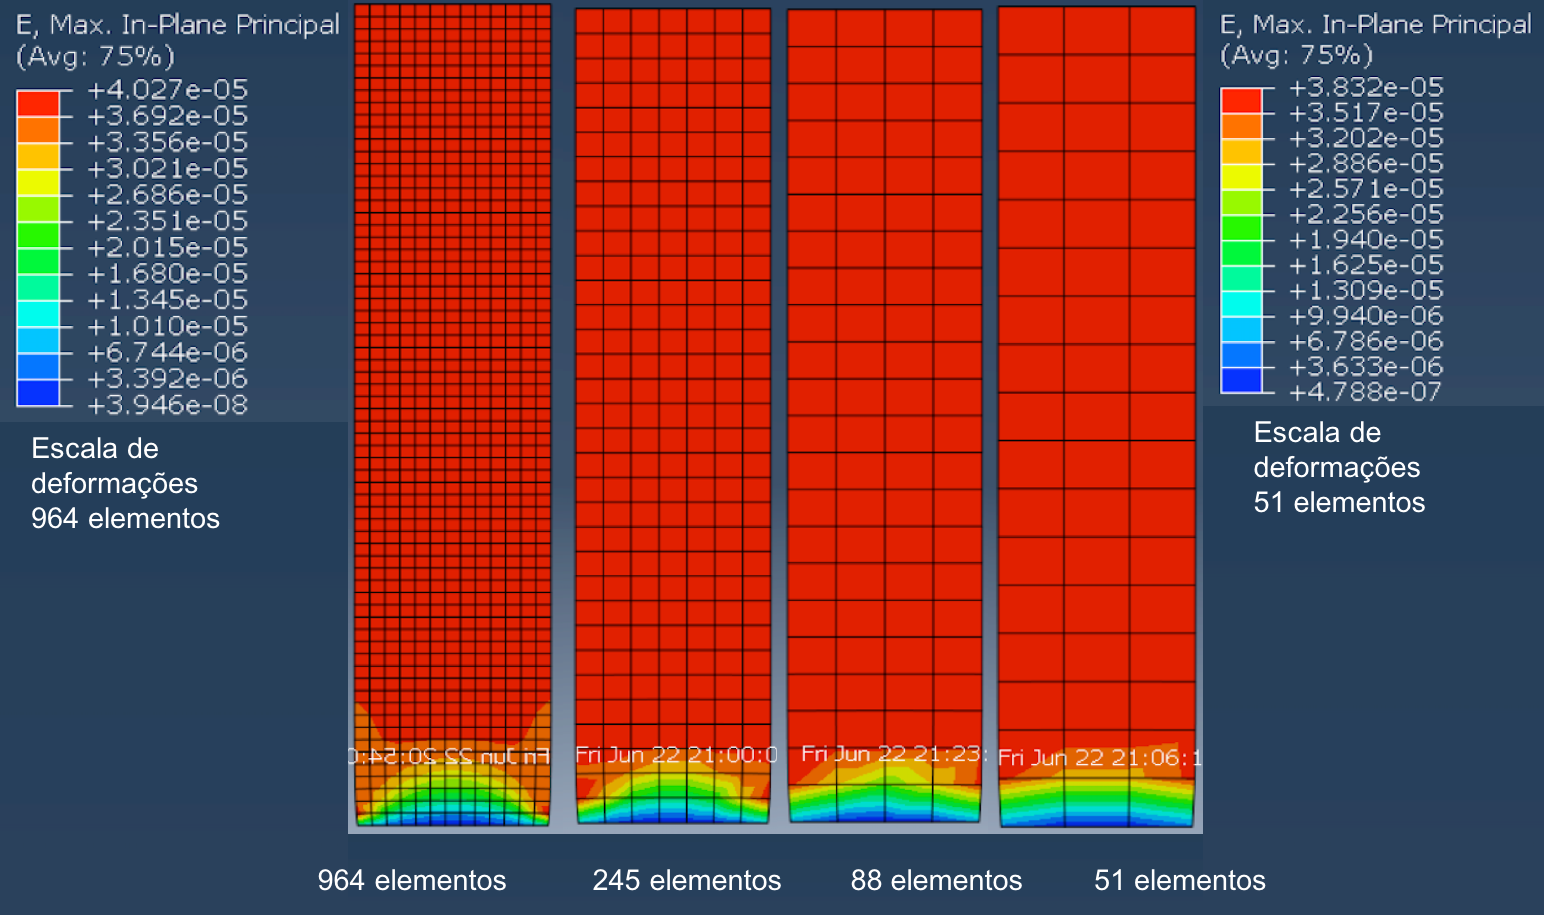
\includegraphics[width=\textwidth,height=\textheight/2,keepaspectratio=true]{strain.png}}
\end{DoxyImageNoCaption}
 

\subsubsection*{T6}

\subsubsection*{html /\+Figuras/stress\+\_\+t6.png}


\begin{DoxyImageNoCaption}
  \mbox{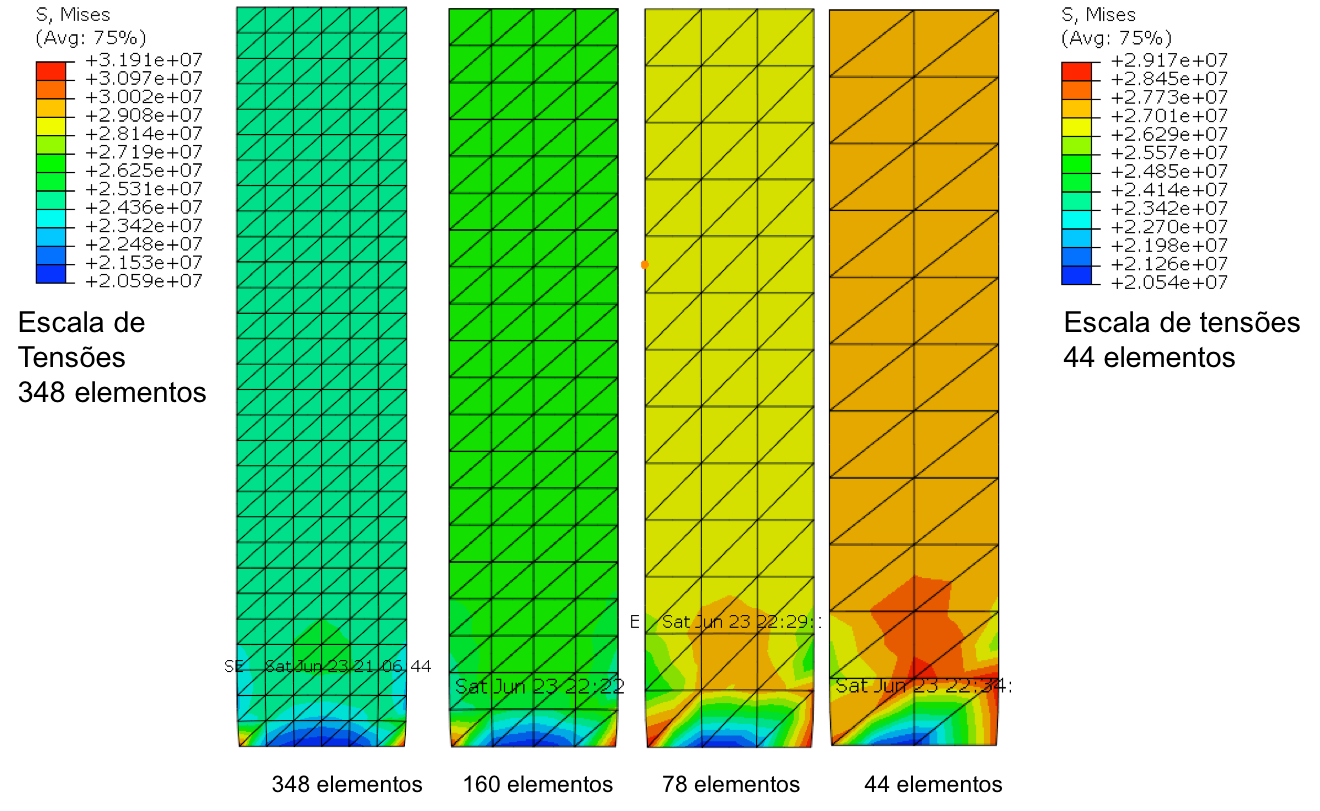
\includegraphics[width=\textwidth,height=\textheight/2,keepaspectratio=true]{stress_t6.png}}
\end{DoxyImageNoCaption}
 

\subsubsection*{html /\+Figuras/strain\+\_\+t6.png}


\begin{DoxyImageNoCaption}
  \mbox{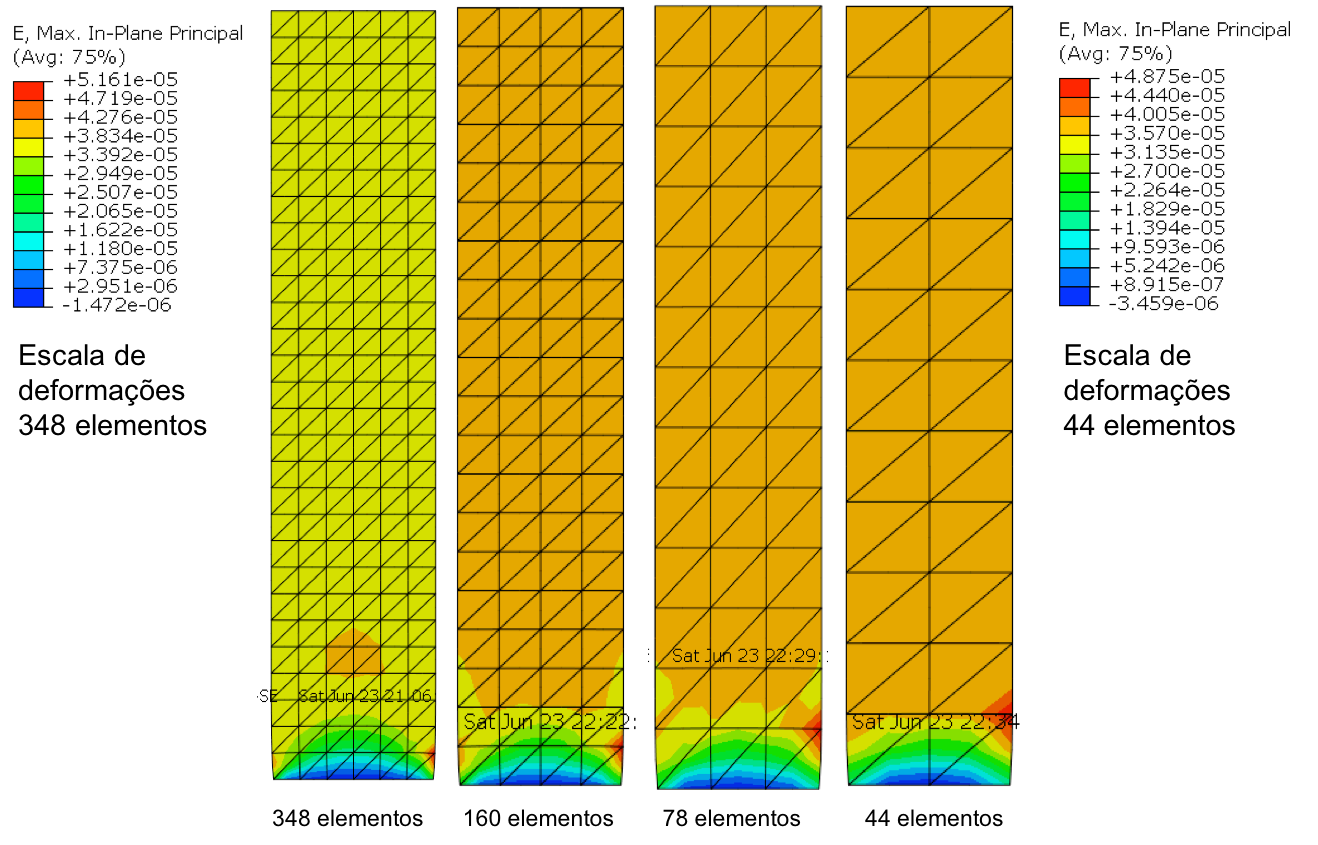
\includegraphics[width=\textwidth,height=\textheight/2,keepaspectratio=true]{strain_t6.png}}
\end{DoxyImageNoCaption}
 

\subsection*{Gráfico Número de Elementos x Tensões Máximas}

\subsubsection*{Q4}

\subsubsection*{html /\+Figuras/q4\+\_\+elementxstress.png}


\begin{DoxyImageNoCaption}
  \mbox{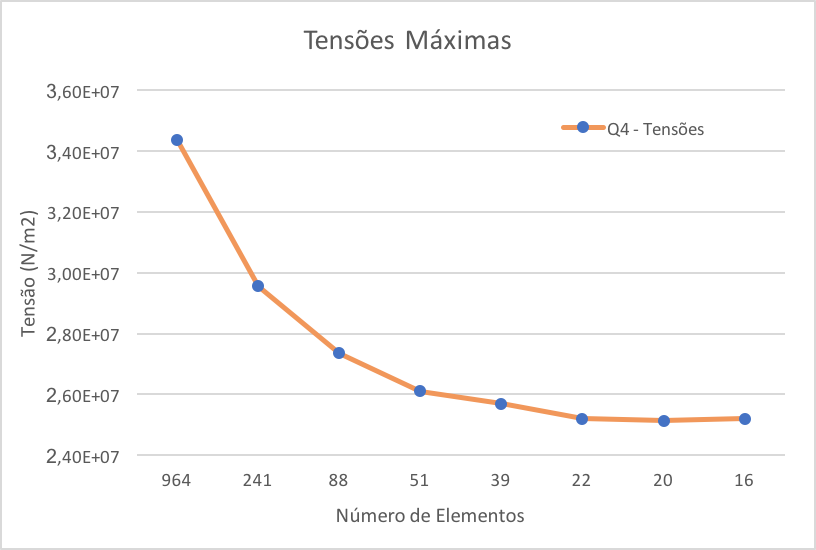
\includegraphics[width=\textwidth,height=\textheight/2,keepaspectratio=true]{q4_elementxstress.png}}
\end{DoxyImageNoCaption}
 

\subsubsection*{T6}

\subsubsection*{html /\+Figuras/t6\+\_\+elementxstress.png}


\begin{DoxyImageNoCaption}
  \mbox{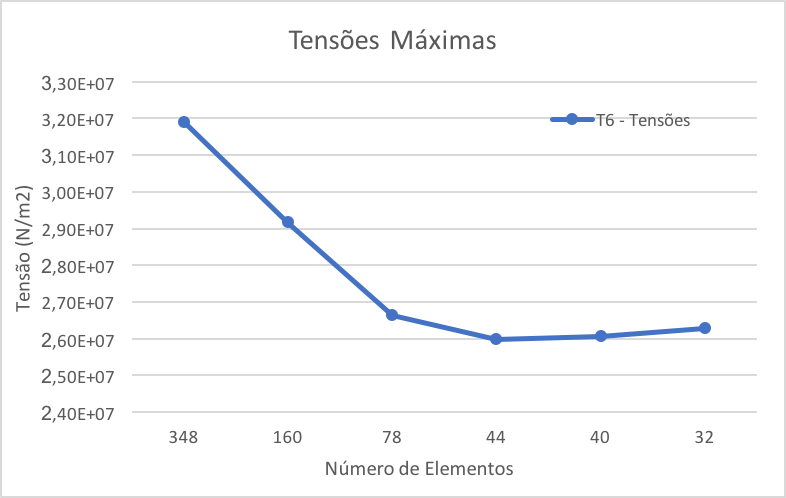
\includegraphics[width=\textwidth,height=\textheight/2,keepaspectratio=true]{t6_elementxstress.png}}
\end{DoxyImageNoCaption}
 

\subsection*{Gráfico Número de Elementos x Deformações Máximas}

\subsubsection*{Q4}

\subsubsection*{html /\+Figuras/q4\+\_\+elementxstrain.png}


\begin{DoxyImageNoCaption}
  \mbox{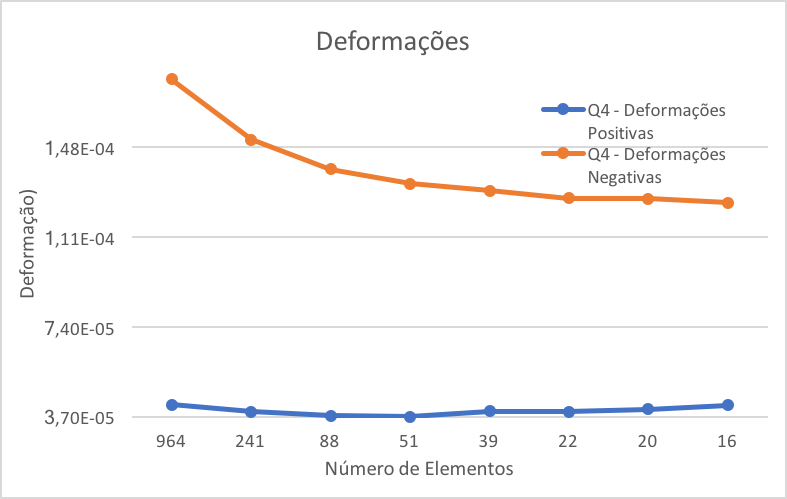
\includegraphics[width=\textwidth,height=\textheight/2,keepaspectratio=true]{q4_elementxstrain.png}}
\end{DoxyImageNoCaption}
 

\subsubsection*{T6}

\subsubsection*{html /\+Figuras/t6\+\_\+elementxstrain.png}


\begin{DoxyImageNoCaption}
  \mbox{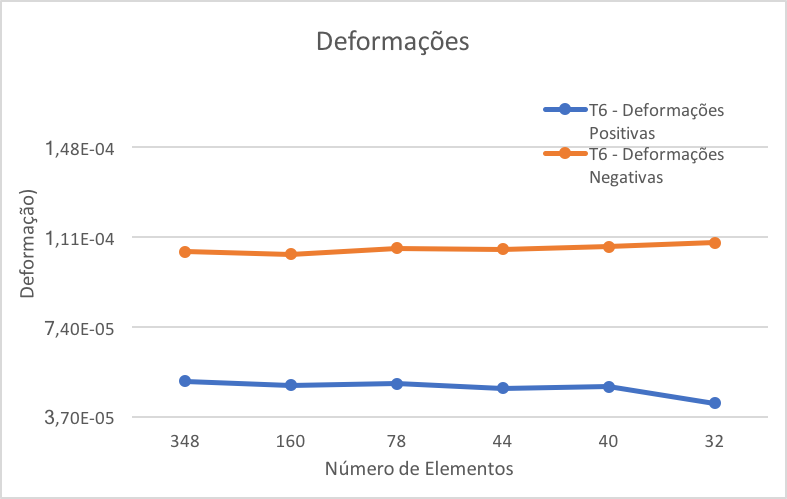
\includegraphics[width=\textwidth,height=\textheight/2,keepaspectratio=true]{t6_elementxstrain.png}}
\end{DoxyImageNoCaption}
 

\section*{Análise dos resultados}


\begin{DoxyItemize}
\item A partir dos resultados, avaliou-\/se a influência do refinamento da malha nos resultados das análises de elementos finitos. Malhas mais refinadas, além de fornecerem resultados com maior grau de suavidade e continuidade, apresentão um comportamento menos rígido em relação as malhas menos refinadas. Apesar de ser uma diferença não tão pronunciada, foi observado que elementos mais refinados tem tanto deformações quanto tensões mais acentuadas.
\item Foi constatado também que, para os elementos do tipo T6, a qualidade da resposta é inferior ao Q4, apesar das funções de interpolação quadrádicas utilizadas.
\end{DoxyItemize}

\subsection*{Referencias até o momento}

\href{http://eigen.tuxfamily.org/index.php?title=IDEs#Visual_Studio}{\tt Eigen Website -\/ Instalation} 
\chapter{Class Index}
\section{Class List}
Here are the classes, structs, unions and interfaces with brief descriptions\+:\begin{DoxyCompactList}
\item\contentsline{section}{\mbox{\hyperlink{classbase_node_class}{base\+Node\+Class$<$ n\+Spatial\+Dimension, numeric\+Type $>$}} }{\pageref{classbase_node_class}}{}
\item\contentsline{section}{\mbox{\hyperlink{classelement_class___q4}{element\+Class\+\_\+\+Q4$<$ numeric\+Type $>$}} }{\pageref{classelement_class___q4}}{}
\end{DoxyCompactList}

\chapter{Class Documentation}
\hypertarget{classbase_node_class}{}\section{base\+Node\+Class$<$ n\+Spatial\+Dimension, numeric\+Type $>$ Class Template Reference}
\label{classbase_node_class}\index{base\+Node\+Class$<$ n\+Spatial\+Dimension, numeric\+Type $>$@{base\+Node\+Class$<$ n\+Spatial\+Dimension, numeric\+Type $>$}}
\subsection*{Public Member Functions}
\begin{DoxyCompactItemize}
\item 
\mbox{\Hypertarget{classbase_node_class_a951ba5f8a8e7082ac978c1a3cffc6ccc}\label{classbase_node_class_a951ba5f8a8e7082ac978c1a3cffc6ccc}} 
{\bfseries base\+Node\+Class} (Eigen\+::\+Matrix$<$ numeric\+Type, n\+Spatial\+Dimension, 1 $>$ position)
\item 
\mbox{\Hypertarget{classbase_node_class_ade0aa681b0ac36364b31a7fcf4b4c295}\label{classbase_node_class_ade0aa681b0ac36364b31a7fcf4b4c295}} 
const Eigen\+::\+Matrix$<$ numeric\+Type, n\+Spatial\+Dimension, 1 $>$ \& {\bfseries get\+M\+\_\+position} () const
\end{DoxyCompactItemize}
\subsection*{Protected Attributes}
\begin{DoxyCompactItemize}
\item 
\mbox{\Hypertarget{classbase_node_class_a68f14d13ea4a416c943f67a60d3107aa}\label{classbase_node_class_a68f14d13ea4a416c943f67a60d3107aa}} 
Eigen\+::\+Matrix$<$ numeric\+Type, n\+Spatial\+Dimension, 1 $>$ {\bfseries m\+\_\+position}
\end{DoxyCompactItemize}


The documentation for this class was generated from the following file\+:\begin{DoxyCompactItemize}
\item 
C\+:/\+Users/igorn/\+Documents/\+Git\+Hub/\+F\+E\+Mproject/base\+Node\+Class.\+hpp\end{DoxyCompactItemize}

\hypertarget{classbase_structural_analysis_class}{}\section{base\+Structural\+Analysis\+Class$<$ numeric\+Type, elem\+Class, node\+Class $>$ Class Template Reference}
\label{classbase_structural_analysis_class}\index{base\+Structural\+Analysis\+Class$<$ numeric\+Type, elem\+Class, node\+Class $>$@{base\+Structural\+Analysis\+Class$<$ numeric\+Type, elem\+Class, node\+Class $>$}}


{\ttfamily \#include $<$base\+Structural\+Analysis\+Class.\+hpp$>$}

\subsection*{Public Member Functions}
\begin{DoxyCompactItemize}
\item 
\mbox{\hyperlink{classbase_structural_analysis_class_a743a6d6c9b29ce5c7e299ed246691b9a}{base\+Structural\+Analysis\+Class}} ()
\item 
\mbox{\hyperlink{classbase_structural_analysis_class_ac51091bf5f718cdc746c20d9cd5a0cab}{base\+Structural\+Analysis\+Class}} (std\+::string file\+Name)
\item 
\mbox{\hyperlink{classbase_structural_analysis_class_a70a5a3407cdeb6f32f69fb1fd7ba6e75}{$\sim$base\+Structural\+Analysis\+Class}} ()
\item 
\mbox{\Hypertarget{classbase_structural_analysis_class_adea296e2d4cafa290794599b62e2abdd}\label{classbase_structural_analysis_class_adea296e2d4cafa290794599b62e2abdd}} 
virtual unsigned int {\bfseries do\+Structural\+Analysis} ()
\item 
\mbox{\Hypertarget{classbase_structural_analysis_class_aa21d6e5d9eea16e4fb57845d93d1ec4b}\label{classbase_structural_analysis_class_aa21d6e5d9eea16e4fb57845d93d1ec4b}} 
virtual bool {\bfseries read\+Formated\+File} (std\+::string file\+Name)
\item 
\mbox{\Hypertarget{classbase_structural_analysis_class_a57fe62169a4032b8c8393d9adb058343}\label{classbase_structural_analysis_class_a57fe62169a4032b8c8393d9adb058343}} 
virtual bool {\bfseries read\+From\+File\+\_\+\+Elem\+List} (std\+::ifstream $\ast$opened\+File)
\item 
\mbox{\Hypertarget{classbase_structural_analysis_class_ad81d20f7c98e21692e68db5019d0e8ae}\label{classbase_structural_analysis_class_ad81d20f7c98e21692e68db5019d0e8ae}} 
virtual bool {\bfseries read\+From\+File\+\_\+\+Node\+List} (std\+::ifstream $\ast$opened\+File)
\item 
\mbox{\Hypertarget{classbase_structural_analysis_class_aa1ca226998df962bc3ea65513da9b938}\label{classbase_structural_analysis_class_aa1ca226998df962bc3ea65513da9b938}} 
virtual bool {\bfseries read\+From\+File\+\_\+\+Material} (std\+::ifstream $\ast$opened\+File)
\item 
\mbox{\Hypertarget{classbase_structural_analysis_class_aca53b1f1642a1dae799df8f906479f93}\label{classbase_structural_analysis_class_aca53b1f1642a1dae799df8f906479f93}} 
virtual Eigen\+::\+Matrix$<$ unsigned int, Eigen\+::\+Dynamic, 1 $>$ {\bfseries compute\+Degrees\+Of\+Freedom} ()
\item 
\mbox{\Hypertarget{classbase_structural_analysis_class_a773fa080feae6b17e47e58e5ed810885}\label{classbase_structural_analysis_class_a773fa080feae6b17e47e58e5ed810885}} 
virtual Eigen\+::\+Sparse\+Matrix$<$ numeric\+Type $>$ {\bfseries evaluate\+Global\+Stiff\+Mat} ()
\item 
\mbox{\Hypertarget{classbase_structural_analysis_class_a8ae8b924f3c1c20f131db1570544cb90}\label{classbase_structural_analysis_class_a8ae8b924f3c1c20f131db1570544cb90}} 
virtual Eigen\+::\+Matrix$<$ numeric\+Type, Eigen\+::\+Dynamic, 1 $>$ {\bfseries evaluate\+Global\+Displac\+Vec} ()
\item 
\mbox{\Hypertarget{classbase_structural_analysis_class_a110e4cdc86a9e8611dade6db8751f02d}\label{classbase_structural_analysis_class_a110e4cdc86a9e8611dade6db8751f02d}} 
virtual Eigen\+::\+Matrix$<$ numeric\+Type, Eigen\+::\+Dynamic, Eigen\+::\+Dynamic $>$ {\bfseries rotation\+Matrix} (Eigen\+::\+Matrix$<$ numeric\+Type, Eigen\+::\+Dynamic, 1 $>$ \&dir\+Elem\+Vec) const =0
\end{DoxyCompactItemize}
\subsection*{Public Attributes}
\begin{DoxyCompactItemize}
\item 
\mbox{\Hypertarget{classbase_structural_analysis_class_ad40dbcb71e338b8cd998ad4bf80fef1a}\label{classbase_structural_analysis_class_ad40dbcb71e338b8cd998ad4bf80fef1a}} 
unsigned int {\bfseries m\+\_\+n\+Dim}
\item 
\mbox{\Hypertarget{classbase_structural_analysis_class_af7ea30f9a3e3c353eeaba07c31c445a0}\label{classbase_structural_analysis_class_af7ea30f9a3e3c353eeaba07c31c445a0}} 
unsigned int {\bfseries m\+\_\+max\+Node\+Deg\+Free}
\item 
\mbox{\Hypertarget{classbase_structural_analysis_class_aed50959156544fc3d15af79eb38d6ae0}\label{classbase_structural_analysis_class_aed50959156544fc3d15af79eb38d6ae0}} 
unsigned int {\bfseries m\+\_\+n\+Node\+Per\+Elem}
\item 
\mbox{\Hypertarget{classbase_structural_analysis_class_abec1d294a55c84f5ef8e227a69d4e5f4}\label{classbase_structural_analysis_class_abec1d294a55c84f5ef8e227a69d4e5f4}} 
unsigned int {\bfseries m\+\_\+n\+Prop\+Per\+Elem}
\item 
\mbox{\Hypertarget{classbase_structural_analysis_class_a9c1dbd7cb8a65f514211505672854330}\label{classbase_structural_analysis_class_a9c1dbd7cb8a65f514211505672854330}} 
unsigned int {\bfseries m\+\_\+n\+Total\+DoF}
\item 
\mbox{\Hypertarget{classbase_structural_analysis_class_a7e59de3567f891a9e6ea32378f0d7435}\label{classbase_structural_analysis_class_a7e59de3567f891a9e6ea32378f0d7435}} 
numeric\+Type {\bfseries m\+\_\+penalty}
\item 
\mbox{\Hypertarget{classbase_structural_analysis_class_a5366e9b75e98f8360ac90c72ea121dcd}\label{classbase_structural_analysis_class_a5366e9b75e98f8360ac90c72ea121dcd}} 
const numeric\+Type {\bfseries m\+\_\+penalty\+\_\+multiplier} = 1e20
\item 
\mbox{\Hypertarget{classbase_structural_analysis_class_a80ad4a3ce359b44670321a7d4cefef58}\label{classbase_structural_analysis_class_a80ad4a3ce359b44670321a7d4cefef58}} 
std\+::vector$<$ elem\+Class $>$ {\bfseries m\+\_\+elem\+List}
\item 
\mbox{\Hypertarget{classbase_structural_analysis_class_a53cf915dc1fc9fcb8ff58b20bfac5632}\label{classbase_structural_analysis_class_a53cf915dc1fc9fcb8ff58b20bfac5632}} 
std\+::vector$<$ unsigned int $>$ {\bfseries m\+\_\+elem\+List\+With\+Pressure\+Applied}
\item 
\mbox{\Hypertarget{classbase_structural_analysis_class_a1007e2a6feb183e4f2aa79cc44eb9bd1}\label{classbase_structural_analysis_class_a1007e2a6feb183e4f2aa79cc44eb9bd1}} 
std\+::vector$<$ node\+Class $>$ {\bfseries m\+\_\+node\+List}
\item 
\mbox{\Hypertarget{classbase_structural_analysis_class_a7a950eab6be3c966121023a6a9797184}\label{classbase_structural_analysis_class_a7a950eab6be3c966121023a6a9797184}} 
std\+::vector$<$ unsigned int $>$ {\bfseries m\+\_\+fixed\+Nodes}
\item 
\mbox{\Hypertarget{classbase_structural_analysis_class_af71b3fd8032c8ac1e177ae6b97a91d1c}\label{classbase_structural_analysis_class_af71b3fd8032c8ac1e177ae6b97a91d1c}} 
std\+::string {\bfseries m\+\_\+file\+Input\+Name}
\item 
\mbox{\Hypertarget{classbase_structural_analysis_class_a610e3e0a3be5e5daa43615f21675b63c}\label{classbase_structural_analysis_class_a610e3e0a3be5e5daa43615f21675b63c}} 
\mbox{\hyperlink{classeigen_linear_solver_info}{eigen\+Linear\+Solver\+Info}} {\bfseries m\+\_\+lin\+Solver\+Info}
\item 
\mbox{\Hypertarget{classbase_structural_analysis_class_a06dce5c9f7beb2873fe6c00c66e985a7}\label{classbase_structural_analysis_class_a06dce5c9f7beb2873fe6c00c66e985a7}} 
numeric\+Type {\bfseries m\+\_\+young\+Modulus}
\item 
\mbox{\Hypertarget{classbase_structural_analysis_class_adacc82b7726291dd9a0a2441863858b4}\label{classbase_structural_analysis_class_adacc82b7726291dd9a0a2441863858b4}} 
numeric\+Type {\bfseries m\+\_\+poisson\+Ratio}
\item 
\mbox{\Hypertarget{classbase_structural_analysis_class_a30c9d240e183d6ed546127192b342086}\label{classbase_structural_analysis_class_a30c9d240e183d6ed546127192b342086}} 
Eigen\+::\+Matrix$<$ unsigned int, Eigen\+::\+Dynamic, 1 $>$ {\bfseries m\+\_\+deg\+Free\+Vec}
\item 
\mbox{\Hypertarget{classbase_structural_analysis_class_a32476178ae646ba8324440cc1d2efd11}\label{classbase_structural_analysis_class_a32476178ae646ba8324440cc1d2efd11}} 
Eigen\+::\+Sparse\+Matrix$<$ numeric\+Type $>$ {\bfseries m\+\_\+glb\+Stiff\+Mat}
\item 
\mbox{\Hypertarget{classbase_structural_analysis_class_a5b4cc2b24256ee92b746ef463f34d035}\label{classbase_structural_analysis_class_a5b4cc2b24256ee92b746ef463f34d035}} 
Eigen\+::\+Matrix$<$ numeric\+Type, Eigen\+::\+Dynamic, 1 $>$ {\bfseries m\+\_\+glbnode\+Force\+Vec}
\item 
\mbox{\Hypertarget{classbase_structural_analysis_class_a9c92d5720fc03e77a2b30a8e5277aeba}\label{classbase_structural_analysis_class_a9c92d5720fc03e77a2b30a8e5277aeba}} 
Eigen\+::\+Matrix$<$ numeric\+Type, Eigen\+::\+Dynamic, 1 $>$ {\bfseries m\+\_\+glb\+Displac\+Vec}
\item 
\mbox{\Hypertarget{classbase_structural_analysis_class_a3497fd3dc60eb8cf056a3d3828000bb2}\label{classbase_structural_analysis_class_a3497fd3dc60eb8cf056a3d3828000bb2}} 
bool {\bfseries m\+\_\+is\+Elem\+List\+Saved}
\item 
\mbox{\Hypertarget{classbase_structural_analysis_class_a9a89aee1ea437bb8f1a633860b306633}\label{classbase_structural_analysis_class_a9a89aee1ea437bb8f1a633860b306633}} 
bool {\bfseries m\+\_\+is\+Node\+List\+Saved}
\item 
\mbox{\Hypertarget{classbase_structural_analysis_class_aeda5815de358a24f99b194854252e94b}\label{classbase_structural_analysis_class_aeda5815de358a24f99b194854252e94b}} 
bool {\bfseries m\+\_\+is\+Initial\+Structure\+Saved}
\item 
\mbox{\Hypertarget{classbase_structural_analysis_class_ad5e1782b128ac071695aae4ee8d7d23a}\label{classbase_structural_analysis_class_ad5e1782b128ac071695aae4ee8d7d23a}} 
bool {\bfseries m\+\_\+is\+Local\+Rotation\+Matrix\+Computed}
\item 
\mbox{\Hypertarget{classbase_structural_analysis_class_a60baf19b10caa39342408548d5a834ac}\label{classbase_structural_analysis_class_a60baf19b10caa39342408548d5a834ac}} 
bool {\bfseries m\+\_\+is\+Degree\+Of\+Freedom\+Vec\+Computed}
\item 
\mbox{\Hypertarget{classbase_structural_analysis_class_af6d2f4bea68e4bd857a2ac6bea8194ec}\label{classbase_structural_analysis_class_af6d2f4bea68e4bd857a2ac6bea8194ec}} 
bool {\bfseries m\+\_\+is\+Glb\+Stiff\+Mat\+Computed}
\item 
\mbox{\Hypertarget{classbase_structural_analysis_class_a779af0fab2226dacec87b0f6a05e1956}\label{classbase_structural_analysis_class_a779af0fab2226dacec87b0f6a05e1956}} 
bool {\bfseries m\+\_\+is\+Glbnode\+Force\+Vec\+Computed}
\item 
\mbox{\Hypertarget{classbase_structural_analysis_class_a920c4ef5aedc3e9bf397c7d67786e696}\label{classbase_structural_analysis_class_a920c4ef5aedc3e9bf397c7d67786e696}} 
bool {\bfseries m\+\_\+is\+Glb\+Displac\+Vec\+Computed}
\item 
\mbox{\Hypertarget{classbase_structural_analysis_class_ac89e923d65f5fc5f8e08d15bf5b65bb5}\label{classbase_structural_analysis_class_ac89e923d65f5fc5f8e08d15bf5b65bb5}} 
bool {\bfseries m\+\_\+is\+Local\+Elem\+Info\+Updated}
\item 
\mbox{\Hypertarget{classbase_structural_analysis_class_a5930a49c82de1cc5d03d0b44788f8af0}\label{classbase_structural_analysis_class_a5930a49c82de1cc5d03d0b44788f8af0}} 
bool {\bfseries m\+\_\+is\+Local\+Node\+Info\+Updated}
\end{DoxyCompactItemize}


\subsection{Detailed Description}
\subsubsection*{template$<$class numeric\+Type, class elem\+Class, class node\+Class$>$\newline
class base\+Structural\+Analysis\+Class$<$ numeric\+Type, elem\+Class, node\+Class $>$}

Structural Analysis superclass to store and compute the analysis. 
\begin{DoxyTemplParams}{Template Parameters}
{\em numeric\+Type} & numeric type to be used, either float or double. \\
\hline
{\em elem\+Class} & Class to be used to store and compute the elements. \\
\hline
{\em node\+Class} & Class to be used to store and compute the nodes. \\
\hline
\end{DoxyTemplParams}


\subsection{Constructor \& Destructor Documentation}
\mbox{\Hypertarget{classbase_structural_analysis_class_a743a6d6c9b29ce5c7e299ed246691b9a}\label{classbase_structural_analysis_class_a743a6d6c9b29ce5c7e299ed246691b9a}} 
\index{base\+Structural\+Analysis\+Class@{base\+Structural\+Analysis\+Class}!base\+Structural\+Analysis\+Class@{base\+Structural\+Analysis\+Class}}
\index{base\+Structural\+Analysis\+Class@{base\+Structural\+Analysis\+Class}!base\+Structural\+Analysis\+Class@{base\+Structural\+Analysis\+Class}}
\subsubsection{\texorpdfstring{base\+Structural\+Analysis\+Class()}{baseStructuralAnalysisClass()}\hspace{0.1cm}{\footnotesize\ttfamily [1/2]}}
{\footnotesize\ttfamily template$<$class numeric\+Type , class elem\+Class , class node\+Class $>$ \\
\mbox{\hyperlink{classbase_structural_analysis_class}{base\+Structural\+Analysis\+Class}}$<$ numeric\+Type, elem\+Class, node\+Class $>$\+::\mbox{\hyperlink{classbase_structural_analysis_class}{base\+Structural\+Analysis\+Class}} (\begin{DoxyParamCaption}{ }\end{DoxyParamCaption})}

Default constructor. \mbox{\Hypertarget{classbase_structural_analysis_class_ac51091bf5f718cdc746c20d9cd5a0cab}\label{classbase_structural_analysis_class_ac51091bf5f718cdc746c20d9cd5a0cab}} 
\index{base\+Structural\+Analysis\+Class@{base\+Structural\+Analysis\+Class}!base\+Structural\+Analysis\+Class@{base\+Structural\+Analysis\+Class}}
\index{base\+Structural\+Analysis\+Class@{base\+Structural\+Analysis\+Class}!base\+Structural\+Analysis\+Class@{base\+Structural\+Analysis\+Class}}
\subsubsection{\texorpdfstring{base\+Structural\+Analysis\+Class()}{baseStructuralAnalysisClass()}\hspace{0.1cm}{\footnotesize\ttfamily [2/2]}}
{\footnotesize\ttfamily template$<$class numeric\+Type , class elem\+Class , class node\+Class $>$ \\
\mbox{\hyperlink{classbase_structural_analysis_class}{base\+Structural\+Analysis\+Class}}$<$ numeric\+Type, elem\+Class, node\+Class $>$\+::\mbox{\hyperlink{classbase_structural_analysis_class}{base\+Structural\+Analysis\+Class}} (\begin{DoxyParamCaption}\item[{std\+::string}]{file\+Name }\end{DoxyParamCaption})\hspace{0.3cm}{\ttfamily [explicit]}}

Read-\/file constructor. 
\begin{DoxyParams}{Parameters}
{\em file\+Name} & Name of the file to be read. \\
\hline
\end{DoxyParams}
\mbox{\Hypertarget{classbase_structural_analysis_class_a70a5a3407cdeb6f32f69fb1fd7ba6e75}\label{classbase_structural_analysis_class_a70a5a3407cdeb6f32f69fb1fd7ba6e75}} 
\index{base\+Structural\+Analysis\+Class@{base\+Structural\+Analysis\+Class}!````~base\+Structural\+Analysis\+Class@{$\sim$base\+Structural\+Analysis\+Class}}
\index{````~base\+Structural\+Analysis\+Class@{$\sim$base\+Structural\+Analysis\+Class}!base\+Structural\+Analysis\+Class@{base\+Structural\+Analysis\+Class}}
\subsubsection{\texorpdfstring{$\sim$base\+Structural\+Analysis\+Class()}{~baseStructuralAnalysisClass()}}
{\footnotesize\ttfamily template$<$class numeric\+Type , class elem\+Class , class node\+Class $>$ \\
\mbox{\hyperlink{classbase_structural_analysis_class}{base\+Structural\+Analysis\+Class}}$<$ numeric\+Type, elem\+Class, node\+Class $>$\+::$\sim$\mbox{\hyperlink{classbase_structural_analysis_class}{base\+Structural\+Analysis\+Class}} (\begin{DoxyParamCaption}{ }\end{DoxyParamCaption})\hspace{0.3cm}{\ttfamily [inline]}}

Default Destructor. 

The documentation for this class was generated from the following file\+:\begin{DoxyCompactItemize}
\item 
C\+:/\+Users/igorn/\+Documents/\+Git\+Hub/\+F\+E\+Mproject/base\+Structural\+Analysis\+Class.\+hpp\end{DoxyCompactItemize}

\hypertarget{classeigen_linear_solver_info}{}\section{eigen\+Linear\+Solver\+Info Class Reference}
\label{classeigen_linear_solver_info}\index{eigen\+Linear\+Solver\+Info@{eigen\+Linear\+Solver\+Info}}


{\ttfamily \#include $<$base\+Structural\+Analysis\+Class.\+hpp$>$}

\subsection*{Public Member Functions}
\begin{DoxyCompactItemize}
\item 
\mbox{\hyperlink{classeigen_linear_solver_info_a7188b8fac261f6f5c2c268fbc4334325}{eigen\+Linear\+Solver\+Info}} ()=default
\item 
void \mbox{\hyperlink{classeigen_linear_solver_info_aeec430481779fd1c759e0f33f0b02c4f}{set\+Values}} (std\+::ptrdiff\+\_\+t iter, double er, Eigen\+::\+Computation\+Info inform)
\end{DoxyCompactItemize}
\subsection*{Public Attributes}
\begin{DoxyCompactItemize}
\item 
\mbox{\Hypertarget{classeigen_linear_solver_info_a74d85f3c4e27ee7caf995c18ac6854a4}\label{classeigen_linear_solver_info_a74d85f3c4e27ee7caf995c18ac6854a4}} 
std\+::ptrdiff\+\_\+t {\bfseries ite}
\item 
\mbox{\Hypertarget{classeigen_linear_solver_info_a752aa62422a4d8ad6cb44d8d56fc6504}\label{classeigen_linear_solver_info_a752aa62422a4d8ad6cb44d8d56fc6504}} 
double {\bfseries error}
\item 
\mbox{\Hypertarget{classeigen_linear_solver_info_a1aecf24673f0238af235b3c80f4c89de}\label{classeigen_linear_solver_info_a1aecf24673f0238af235b3c80f4c89de}} 
Eigen\+::\+Computation\+Info {\bfseries info}
\end{DoxyCompactItemize}


\subsection{Detailed Description}
Simple structure to stores a linear system solution by Eigen lib. 

\subsection{Constructor \& Destructor Documentation}
\mbox{\Hypertarget{classeigen_linear_solver_info_a7188b8fac261f6f5c2c268fbc4334325}\label{classeigen_linear_solver_info_a7188b8fac261f6f5c2c268fbc4334325}} 
\index{eigen\+Linear\+Solver\+Info@{eigen\+Linear\+Solver\+Info}!eigen\+Linear\+Solver\+Info@{eigen\+Linear\+Solver\+Info}}
\index{eigen\+Linear\+Solver\+Info@{eigen\+Linear\+Solver\+Info}!eigen\+Linear\+Solver\+Info@{eigen\+Linear\+Solver\+Info}}
\subsubsection{\texorpdfstring{eigen\+Linear\+Solver\+Info()}{eigenLinearSolverInfo()}}
{\footnotesize\ttfamily eigen\+Linear\+Solver\+Info\+::eigen\+Linear\+Solver\+Info (\begin{DoxyParamCaption}{ }\end{DoxyParamCaption})\hspace{0.3cm}{\ttfamily [default]}}

Default constructor 

\subsection{Member Function Documentation}
\mbox{\Hypertarget{classeigen_linear_solver_info_aeec430481779fd1c759e0f33f0b02c4f}\label{classeigen_linear_solver_info_aeec430481779fd1c759e0f33f0b02c4f}} 
\index{eigen\+Linear\+Solver\+Info@{eigen\+Linear\+Solver\+Info}!set\+Values@{set\+Values}}
\index{set\+Values@{set\+Values}!eigen\+Linear\+Solver\+Info@{eigen\+Linear\+Solver\+Info}}
\subsubsection{\texorpdfstring{set\+Values()}{setValues()}}
{\footnotesize\ttfamily void eigen\+Linear\+Solver\+Info\+::set\+Values (\begin{DoxyParamCaption}\item[{std\+::ptrdiff\+\_\+t}]{iter,  }\item[{double}]{er,  }\item[{Eigen\+::\+Computation\+Info}]{inform }\end{DoxyParamCaption})\hspace{0.3cm}{\ttfamily [inline]}}

Setter method 
\begin{DoxyParams}{Parameters}
{\em iter} & Number of iterations. \\
\hline
{\em er} & Estimated error. \\
\hline
{\em inform} & Information about the solution process. \\
\hline
\end{DoxyParams}


The documentation for this class was generated from the following file\+:\begin{DoxyCompactItemize}
\item 
C\+:/\+Users/igorn/\+Documents/\+Git\+Hub/\+F\+E\+Mproject/base\+Structural\+Analysis\+Class.\+hpp\end{DoxyCompactItemize}

\hypertarget{classelement_class___q4}{}\section{element\+Class\+\_\+\+Q4$<$ numeric\+Type $>$ Class Template Reference}
\label{classelement_class___q4}\index{element\+Class\+\_\+\+Q4$<$ numeric\+Type $>$@{element\+Class\+\_\+\+Q4$<$ numeric\+Type $>$}}


{\ttfamily \#include $<$element\+Class\+\_\+\+Q4.\+hpp$>$}

\subsection*{Public Member Functions}
\begin{DoxyCompactItemize}
\item 
\mbox{\Hypertarget{classelement_class___q4_a394807d1b7b587bdf8a9fef0ad207cb0}\label{classelement_class___q4_a394807d1b7b587bdf8a9fef0ad207cb0}} 
\mbox{\hyperlink{classelement_class___q4_a394807d1b7b587bdf8a9fef0ad207cb0}{element\+Class\+\_\+\+Q4}} ()
\begin{DoxyCompactList}\small\item\em Default Constructor. \end{DoxyCompactList}\item 
\mbox{\Hypertarget{classelement_class___q4_a26cbfc05c8238f05269a7a596bed8264}\label{classelement_class___q4_a26cbfc05c8238f05269a7a596bed8264}} 
\mbox{\hyperlink{classelement_class___q4_a26cbfc05c8238f05269a7a596bed8264}{element\+Class\+\_\+\+Q4}} (const std\+::vector$<$ unsigned int $>$ \&nodal\+Connectivity, const Eigen\+::\+Matrix$<$ numeric\+Type, 4, 2 $>$ \&nodal\+Pos\+Coord)
\begin{DoxyCompactList}\small\item\em General Constructor. \end{DoxyCompactList}\item 
Eigen\+::\+Sparse\+Matrix$<$ numeric\+Type $>$ \mbox{\hyperlink{classelement_class___q4_adc47e0786349f327fe45e3744080d3c5}{spr\+MatN}} (const Matrix$<$ numeric\+Type, 2, 1 $>$ \&position\+Vec) const
\item 
Eigen\+::\+Sparse\+Matrix$<$ numeric\+Type $>$ \mbox{\hyperlink{classelement_class___q4_a7503f92c139700e19433c2843496b670}{spr\+MatB}} (const Matrix$<$ numeric\+Type, 2, 1 $>$ \&position\+Vec) const
\item 
Eigen\+::\+Sparse\+Matrix$<$ numeric\+Type $>$ \mbox{\hyperlink{classelement_class___q4_a0063f8e857239df14972ebcd95b9cdca}{spr\+MatK}} () const
\item 
const vector$<$ unsigned int $>$ \& \mbox{\hyperlink{classelement_class___q4_aa6a26e36d49ce1008285cf9eb6ef4748}{get\+M\+\_\+nodal\+Connectivity}} () const
\end{DoxyCompactItemize}


\subsection{Detailed Description}
\subsubsection*{template$<$class numeric\+Type$>$\newline
class element\+Class\+\_\+\+Q4$<$ numeric\+Type $>$}

Q4 Isoparametric Element Class. 
\begin{DoxyTemplParams}{Template Parameters}
{\em numeric\+Type} & numeric type to be used, either float or double. \\
\hline
\end{DoxyTemplParams}


\subsection{Member Function Documentation}
\mbox{\Hypertarget{classelement_class___q4_aa6a26e36d49ce1008285cf9eb6ef4748}\label{classelement_class___q4_aa6a26e36d49ce1008285cf9eb6ef4748}} 
\index{element\+Class\+\_\+\+Q4@{element\+Class\+\_\+\+Q4}!get\+M\+\_\+nodal\+Connectivity@{get\+M\+\_\+nodal\+Connectivity}}
\index{get\+M\+\_\+nodal\+Connectivity@{get\+M\+\_\+nodal\+Connectivity}!element\+Class\+\_\+\+Q4@{element\+Class\+\_\+\+Q4}}
\subsubsection{\texorpdfstring{get\+M\+\_\+nodal\+Connectivity()}{getM\_nodalConnectivity()}}
{\footnotesize\ttfamily template$<$class numeric\+Type $>$ \\
const vector$<$ unsigned int $>$ \& \mbox{\hyperlink{classelement_class___q4}{element\+Class\+\_\+\+Q4}}$<$ numeric\+Type $>$\+::get\+M\+\_\+nodal\+Connectivity (\begin{DoxyParamCaption}{ }\end{DoxyParamCaption}) const}

Getter Method\+: Get the identificators of all nodes of this element. \begin{DoxyReturn}{Returns}
the identificators of all nodes of this element. 
\end{DoxyReturn}
\mbox{\Hypertarget{classelement_class___q4_a7503f92c139700e19433c2843496b670}\label{classelement_class___q4_a7503f92c139700e19433c2843496b670}} 
\index{element\+Class\+\_\+\+Q4@{element\+Class\+\_\+\+Q4}!spr\+MatB@{spr\+MatB}}
\index{spr\+MatB@{spr\+MatB}!element\+Class\+\_\+\+Q4@{element\+Class\+\_\+\+Q4}}
\subsubsection{\texorpdfstring{spr\+Mat\+B()}{sprMatB()}}
{\footnotesize\ttfamily template$<$class numeric\+Type $>$ \\
Eigen\+::\+Sparse\+Matrix$<$ numeric\+Type $>$ \mbox{\hyperlink{classelement_class___q4}{element\+Class\+\_\+\+Q4}}$<$ numeric\+Type $>$\+::spr\+MatB (\begin{DoxyParamCaption}\item[{const Matrix$<$ numeric\+Type, 2, 1 $>$ \&}]{position\+Vec }\end{DoxyParamCaption}) const}

Method\+: Get interpolation function derivatives of the isoparametric element. It returns the uncompressed format. 
\begin{DoxyParams}{Parameters}
{\em position\+Vec} & Position Vector of a point inside the element (to interpolate). \\
\hline
\end{DoxyParams}
\begin{DoxyReturn}{Returns}
Returns B (uncompressed version)\+: A sparse matrix with the derivatives of the isoparametric element. B(3,4); 
\end{DoxyReturn}
\mbox{\Hypertarget{classelement_class___q4_a0063f8e857239df14972ebcd95b9cdca}\label{classelement_class___q4_a0063f8e857239df14972ebcd95b9cdca}} 
\index{element\+Class\+\_\+\+Q4@{element\+Class\+\_\+\+Q4}!spr\+MatK@{spr\+MatK}}
\index{spr\+MatK@{spr\+MatK}!element\+Class\+\_\+\+Q4@{element\+Class\+\_\+\+Q4}}
\subsubsection{\texorpdfstring{spr\+Mat\+K()}{sprMatK()}}
{\footnotesize\ttfamily template$<$class numeric\+Type $>$ \\
Eigen\+::\+Sparse\+Matrix$<$ numeric\+Type $>$ \mbox{\hyperlink{classelement_class___q4}{element\+Class\+\_\+\+Q4}}$<$ numeric\+Type $>$\+::spr\+MatK (\begin{DoxyParamCaption}{ }\end{DoxyParamCaption}) const}

Method\+: Evaluate the local stiffness matrix of the element. \begin{DoxyReturn}{Returns}
local stiffness matrix of the element. 
\end{DoxyReturn}
\mbox{\Hypertarget{classelement_class___q4_adc47e0786349f327fe45e3744080d3c5}\label{classelement_class___q4_adc47e0786349f327fe45e3744080d3c5}} 
\index{element\+Class\+\_\+\+Q4@{element\+Class\+\_\+\+Q4}!spr\+MatN@{spr\+MatN}}
\index{spr\+MatN@{spr\+MatN}!element\+Class\+\_\+\+Q4@{element\+Class\+\_\+\+Q4}}
\subsubsection{\texorpdfstring{spr\+Mat\+N()}{sprMatN()}}
{\footnotesize\ttfamily template$<$class numeric\+Type $>$ \\
Eigen\+::\+Sparse\+Matrix$<$ numeric\+Type $>$ \mbox{\hyperlink{classelement_class___q4}{element\+Class\+\_\+\+Q4}}$<$ numeric\+Type $>$\+::spr\+MatN (\begin{DoxyParamCaption}\item[{const Matrix$<$ numeric\+Type, 2, 1 $>$ \&}]{position\+Vec }\end{DoxyParamCaption}) const}

Method\+: Get interpolation functions of the isoparametric element. It returns the uncompressed format. 
\begin{DoxyParams}{Parameters}
{\em position\+Vec} & Position Vector of a point inside the element (to interpolate). \\
\hline
\end{DoxyParams}
\begin{DoxyReturn}{Returns}
Returns N (uncompressed version)\+: Represents the nodal interpolation functions of the isoparametric element. N(2,4); 
\end{DoxyReturn}


The documentation for this class was generated from the following file\+:\begin{DoxyCompactItemize}
\item 
C\+:/\+Users/igorn/\+Documents/\+Git\+Hub/\+F\+E\+Mproject/element\+Class\+\_\+\+Q4.\+hpp\end{DoxyCompactItemize}

\hypertarget{classelement_class___t6}{}\section{element\+Class\+\_\+\+T6$<$ numeric\+Type $>$ Class Template Reference}
\label{classelement_class___t6}\index{element\+Class\+\_\+\+T6$<$ numeric\+Type $>$@{element\+Class\+\_\+\+T6$<$ numeric\+Type $>$}}


{\ttfamily \#include $<$element\+Class\+\_\+\+T6.\+hpp$>$}

\subsection*{Public Member Functions}
\begin{DoxyCompactItemize}
\item 
\mbox{\Hypertarget{classelement_class___t6_ae5cf7beb6805a64e843bde5b86411ba1}\label{classelement_class___t6_ae5cf7beb6805a64e843bde5b86411ba1}} 
\mbox{\hyperlink{classelement_class___t6_ae5cf7beb6805a64e843bde5b86411ba1}{element\+Class\+\_\+\+T6}} ()
\begin{DoxyCompactList}\small\item\em Default Constructor. \end{DoxyCompactList}\item 
\mbox{\Hypertarget{classelement_class___t6_ac18008e975c7da2a42eb2b952c335faf}\label{classelement_class___t6_ac18008e975c7da2a42eb2b952c335faf}} 
\mbox{\hyperlink{classelement_class___t6_ac18008e975c7da2a42eb2b952c335faf}{element\+Class\+\_\+\+T6}} (numeric\+Type young\+Modulus, numeric\+Type poisson\+Ratio, const std\+::vector$<$ unsigned int $>$ \&nodal\+Connectivity, const Eigen\+::\+Matrix$<$ numeric\+Type, 6, 2 $>$ \&nodal\+Pos\+Coord)
\begin{DoxyCompactList}\small\item\em General Constructor. \end{DoxyCompactList}\item 
Eigen\+::\+Sparse\+Matrix$<$ numeric\+Type $>$ \mbox{\hyperlink{classelement_class___t6_ad8f57028dfbb4215979ef16b88d65957}{spr\+MatN}} (const Matrix$<$ numeric\+Type, 2, 1 $>$ \&position\+Vec) const
\item 
Eigen\+::\+Sparse\+Matrix$<$ numeric\+Type $>$ \mbox{\hyperlink{classelement_class___t6_a03adb5b9a48edd11f48d1749e388ab40}{spr\+MatB}} (const Matrix$<$ numeric\+Type, 2, 1 $>$ \&position\+Vec) const
\item 
Eigen\+::\+Sparse\+Matrix$<$ numeric\+Type $>$ \mbox{\hyperlink{classelement_class___t6_a7f9d1575134a4afe28a5505ce4e6de4d}{spr\+MatK}} () const
\item 
const std\+::vector$<$ unsigned int $>$ \& \mbox{\hyperlink{classelement_class___t6_aee26f002dd5cc8d34f03e7ef008a7208}{get\+M\+\_\+nodal\+Connectivity}} () const
\end{DoxyCompactItemize}


\subsection{Detailed Description}
\subsubsection*{template$<$class numeric\+Type$>$\newline
class element\+Class\+\_\+\+T6$<$ numeric\+Type $>$}

T6 Isoparametric Element Class. 
\begin{DoxyTemplParams}{Template Parameters}
{\em numeric\+Type} & numeric type to be used, either float or double. \\
\hline
\end{DoxyTemplParams}


\subsection{Member Function Documentation}
\mbox{\Hypertarget{classelement_class___t6_aee26f002dd5cc8d34f03e7ef008a7208}\label{classelement_class___t6_aee26f002dd5cc8d34f03e7ef008a7208}} 
\index{element\+Class\+\_\+\+T6@{element\+Class\+\_\+\+T6}!get\+M\+\_\+nodal\+Connectivity@{get\+M\+\_\+nodal\+Connectivity}}
\index{get\+M\+\_\+nodal\+Connectivity@{get\+M\+\_\+nodal\+Connectivity}!element\+Class\+\_\+\+T6@{element\+Class\+\_\+\+T6}}
\subsubsection{\texorpdfstring{get\+M\+\_\+nodal\+Connectivity()}{getM\_nodalConnectivity()}}
{\footnotesize\ttfamily template$<$class numeric\+Type $>$ \\
const std\+::vector$<$ unsigned int $>$ \& \mbox{\hyperlink{classelement_class___t6}{element\+Class\+\_\+\+T6}}$<$ numeric\+Type $>$\+::get\+M\+\_\+nodal\+Connectivity (\begin{DoxyParamCaption}{ }\end{DoxyParamCaption}) const}

Getter Method\+: Get the identificators of all nodes of this element. \begin{DoxyReturn}{Returns}
the identificators of all nodes of this element. 
\end{DoxyReturn}
\mbox{\Hypertarget{classelement_class___t6_a03adb5b9a48edd11f48d1749e388ab40}\label{classelement_class___t6_a03adb5b9a48edd11f48d1749e388ab40}} 
\index{element\+Class\+\_\+\+T6@{element\+Class\+\_\+\+T6}!spr\+MatB@{spr\+MatB}}
\index{spr\+MatB@{spr\+MatB}!element\+Class\+\_\+\+T6@{element\+Class\+\_\+\+T6}}
\subsubsection{\texorpdfstring{spr\+Mat\+B()}{sprMatB()}}
{\footnotesize\ttfamily template$<$class numeric\+Type $>$ \\
Eigen\+::\+Sparse\+Matrix$<$ numeric\+Type $>$ \mbox{\hyperlink{classelement_class___t6}{element\+Class\+\_\+\+T6}}$<$ numeric\+Type $>$\+::spr\+MatB (\begin{DoxyParamCaption}\item[{const Matrix$<$ numeric\+Type, 2, 1 $>$ \&}]{position\+Vec }\end{DoxyParamCaption}) const}

Method\+: Get interpolation function derivatives of the isoparametric element. It returns the uncompressed format. 
\begin{DoxyParams}{Parameters}
{\em position\+Vec} & Position Vector of a point inside the element (to interpolate). \\
\hline
\end{DoxyParams}
\begin{DoxyReturn}{Returns}
Returns B (uncompressed version)\+: A sparse matrix with the derivatives of the isoparametric element. B(3,6); 
\end{DoxyReturn}
\mbox{\Hypertarget{classelement_class___t6_a7f9d1575134a4afe28a5505ce4e6de4d}\label{classelement_class___t6_a7f9d1575134a4afe28a5505ce4e6de4d}} 
\index{element\+Class\+\_\+\+T6@{element\+Class\+\_\+\+T6}!spr\+MatK@{spr\+MatK}}
\index{spr\+MatK@{spr\+MatK}!element\+Class\+\_\+\+T6@{element\+Class\+\_\+\+T6}}
\subsubsection{\texorpdfstring{spr\+Mat\+K()}{sprMatK()}}
{\footnotesize\ttfamily template$<$class numeric\+Type $>$ \\
Eigen\+::\+Sparse\+Matrix$<$ numeric\+Type $>$ \mbox{\hyperlink{classelement_class___t6}{element\+Class\+\_\+\+T6}}$<$ numeric\+Type $>$\+::spr\+MatK (\begin{DoxyParamCaption}{ }\end{DoxyParamCaption}) const}

Method\+: Evaluate the local stiffness matrix of the element. \begin{DoxyReturn}{Returns}
local stiffness matrix of the element. 
\end{DoxyReturn}
\mbox{\Hypertarget{classelement_class___t6_ad8f57028dfbb4215979ef16b88d65957}\label{classelement_class___t6_ad8f57028dfbb4215979ef16b88d65957}} 
\index{element\+Class\+\_\+\+T6@{element\+Class\+\_\+\+T6}!spr\+MatN@{spr\+MatN}}
\index{spr\+MatN@{spr\+MatN}!element\+Class\+\_\+\+T6@{element\+Class\+\_\+\+T6}}
\subsubsection{\texorpdfstring{spr\+Mat\+N()}{sprMatN()}}
{\footnotesize\ttfamily template$<$class numeric\+Type $>$ \\
Eigen\+::\+Sparse\+Matrix$<$ numeric\+Type $>$ \mbox{\hyperlink{classelement_class___t6}{element\+Class\+\_\+\+T6}}$<$ numeric\+Type $>$\+::spr\+MatN (\begin{DoxyParamCaption}\item[{const Matrix$<$ numeric\+Type, 2, 1 $>$ \&}]{position\+Vec }\end{DoxyParamCaption}) const}

Method\+: Get interpolation functions of the isoparametric element. It returns the uncompressed format. 
\begin{DoxyParams}{Parameters}
{\em position\+Vec} & Position Vector of a point inside the element (to interpolate). \\
\hline
\end{DoxyParams}
\begin{DoxyReturn}{Returns}
Returns N (uncompressed version)\+: Represents the nodal interpolation functions of the isoparametric element. N(2,6); 
\end{DoxyReturn}


The documentation for this class was generated from the following file\+:\begin{DoxyCompactItemize}
\item 
C\+:/\+Users/igorn/\+Documents/\+Git\+Hub/\+F\+E\+Mproject/element\+Class\+\_\+\+T6.\+hpp\end{DoxyCompactItemize}

%--- End generated contents ---

% Index
\backmatter
\newpage
\phantomsection
\clearemptydoublepage
\addcontentsline{toc}{chapter}{Index}
\printindex

\end{document}
